
\documentclass[11pt]{article}
\usepackage[ngerman]{babel}
\usepackage{times}
\usepackage{url}
\usepackage{latexsym}
\usepackage[utf8]{inputenc}  %% to get umlauts right
\usepackage{graphicx}
\usepackage{covington}
\usepackage[onehalfspacing]{setspace}

\usepackage{breakcites}
 
\setlength{\topmargin}{-1cm}
\setlength{\textheight}{23cm}
\setlength{\oddsidemargin}{0.0cm}
\setlength{\textwidth}{16cm}


\pagestyle{myheadings}    % Go for customized headings
\markboth{Test}{Gonzalo Suazo: MÜ nach "SimpleSpanish" und Alignierung \hspace{2cm} \today \hfill }


\begin{document}


\begin{titlepage}

\includegraphics[height=20mm]{uzh_logo_d_pos}\\
\begin{center}

{\sffamily
Seminar \\
\textbf{Automatische Textvereinfachung} \\
Herbstsemester 2019 \\

\vspace{2cm}

{\Huge Analyse von übersetztem SimpleEnglish Wikipedia nach Spanisch und dessen Alignierung}\\

\vspace{4cm}

\textbf{Verfasser: Gonzalo Suazo} \\
	Matrikel-Nr: 06-726-672 \\

\vspace{2cm}

Dozenten:  Martin Volk, Sarah Ebling



Institut f\"ur Computerlinguistik

\vfill Abgabedatum: 17.01.2020

\vspace{3cm}
}
\end{center}

\end{titlepage}

\newpage



% \begin{abstract}
% The abstract goes here, if you want to use it. It is optional ...
% \end{abstract}


\section{Einführung}
\subsection{Motivation}
SimpleEnglish Wikipedia Artikel sind speziell in vereinfachter, Leichter Sprache geschrieben worden, um Personen mit kognitiven 
Einschränkungen, das Verständnis solcher Texte zu vereinfachen. Die Betroffenen Personen, sollen einen vereinfachten Zugang zur Information erhalten und so die Inklusion voranzutreiben. 

Trotz mehrmaligen versuchen, die SimpleEnglish Wikipedia in anderen Sprachen zu portieren, wurden alle diese Anträge verworfen. Nach heutigem Stand, gibt es keine vereinfachte Wikipedia in anderen Sprachen, ausser in Englisch.
\subsection{Fragestellungen und Ziele des Seminarprojekts}

Dieses Seminarprojekt geht es darum, in SimpleEnglish den Text nach Spanisch zu übersetzen, die Ergebnisse auszuwerten  und zum Schluss, die Texte alignieren zu lassen mit CATS. 
\newline In einem zweiten Schritt, wurden die Texte miteinander aligniert. Dazu abe ich die Text in "SimpleSpanish" und originaler spanischer Wikipdia miteinander aligniert, mittels \textit{CATS}, einem Tool für die automatische Textvereinfachung. Dabei sind einige Faktoren zu beachten, die in verschiedensprachigen Wikipedia-Artikeln der Fall ist, ob die Themen der Artikel semantisch überlappen oder nicht.
\newline\newline Die Fragen, die sich in diesem Kontext aufdrängen sind: 
\newline\begin{enumerate}
\item \textbf{Was passiert, wenn ich ein übersetztes SimpleEnglish-Wikipedia Artikel --in diesem konkreten Fall die Übersetzung nach Spanisch-- automatisch auch ein vereinfachter Text in der Zielsprache? }
\item \textbf{Wenn man die Alignierung zwischen Artikeln in "SimpleSpanish" und originaler spanischer Wiki-pedia analysiert -- kann von einem parallelem Corpus "SimpleSpanish"--ES gesprochen werden? }
\end{enumerate}

\section{Verwandte Arbeiten}
\subsection{Leichte Sprache -- \textit{Lectura fácil}}
In der Iberischen Halbinsel, sind vereinzelte Institutionen kreiert worden, um Personen mit kognitiven Schwierigkeiten, in den Alltag zu integrieren. Wichtig zu nennen sind hier die Institution \textit{Plena Inclusión}\footnote{https://www.plenainclusion.org/} , die 1964 unter dem Namen \textit{FEAPS} - \textit{Federación Española de Asociaciones Pro Subnormales} - gegründet wurde. Es handelt sich dabei um ein Netzwerk von Organisationen, das sich um die Einhaltung der Rechte von Menschen kognitiven Einschränkungen kümmert.

\textit{Associació Lectura Fácil} (ALF) \footnote{http://www.lecturafacil.net/}, die in Barcelona 2003 gegründet wurde, kümmert sich um die Lektüre von Büchern in Leichter Sprache. Diese Institution hat 270 Bücher in Leichter Sprache produziert und 150 Kurse rund um das Thema der vereinfachten Sprache gehalten. Zudem beinhaltet die Institution 500 Leseklubs, für die gemeinsame Lektüre und Erarbeitung von literarischen Texten in Leichter Sprache.

\subsection{Automatische Textvereinfachng }
Ausserdem wurde das Projekt \textit{Simplext}\footnote{http://simplext.taln.upf.edu/} ins Leben gerufen, um die automatische Textvereinfachung von Nachrichtenseiten, welche auf mobilen Endgeräten gelesen werden können. Weil Texte von Nach- richten derart volatil sind, muss man eine automatisierte Methode finden, um die Texte zu vereinfachen, denn manuelles Vereinfachen benötigt zu viel Zeit. Es handelt sich dabei um eine lexikalische und syntaktische Vereinfachung. Dieser hybride Ansatz, verwendet einen statistischen Classifier, der entscheidet, ob vereinfacht werden soll oder nicht. Dabei handelt es sich um einen regelbasierten Ansatz. Die betroffenen Personen, können so die Texte in elektronischer Form, schnell und unkompliziert in Leichter Sprache lesen. 

\section{Regelwerke in Leichter Sprache: \textit{Lectura fácil}}
Um einen Überblick in die Erforschung der Leichten Sprache in der iberischen Halbinsel zu erhalten und um Grundlegende Unterschieden zu den deutschsprachigen Regelwerken zu erhalten, habe ich dafür zwei Bücher gelesen, welche die vereinfachen Texte in Spanisch behandeln.

Das erste Buch ist von Inclusion Europe -- \textit{Información para todos} \cite{europe2010informacion} -- und ist in Leichter Sprache geschrieben. Dieser Leitfaden, ist mehr eine Anleitung für Menschen mit kognitiven Einschränkungen, damit sie klar und kompakt in Erfahrung bringen können, was Leichte Sprache ist und wie sie diese Konzepte anwenden können. Auch ist dieses Buch für Leute gedacht, die andere Personen mit den gleichen kognitiven Defiziten, die Leichte Sprache näher bringen können. Auf diese Weise, kann das Volk auch einfache Weise informiert werden, was diese vereinfachte Sprache genau ist und wie sie angewendet werden kann. 

Das zweite Buch -- \textit{Lectura fácil: Métodos de redacción y evaluación} \cite{garcia2014lectura} -- ist mehr wissenschaftlicher Art, denn es beschreibt die gleichen Konzepte auf ausführlichere Weise. Dieses Regelwerk ist einerseits für Schriftsteller gedacht, die Texte in Leichter Sprache verfassen wollen und Linguisten gedacht, die sich wissenschaftlich mit der Leichten Sprache befassen und mehr lernen wollen und diese Konzepte in wissenschaftlichen Publikationen weitergeben möchten. Dieses Buch bleibt nicht nur auf der redaktionellen Ebene, sondern beschreibt mehrere Methoden zur Evaluation der Leichten Sprache in hispanischer Sprache. Es behandelt auch Punkte, wie der der Erstellung von Büchern, zum Beispiel, wie viele Zeilen eine Seite in einem Buch enthalten soll und wie viele Zeichen ein Satz im Idealfall enthalten soll, damit es noch in die Kategorie der Leichten Sprache aufgenommen werden kann.

\subsection{Signifikante Unterschiede mit den Regelwerken im deutschen Raum}
TODO: Beschreiben einiger Unterschiede mit Regelwerken der Leichten Sprache.
TODO: Einige Sätze im Detail analysieren.
TODO: Durchschnitt und Varianz berechnen

\section{Methodologie}
Meine gewählte Methodologie für dieses Seminarprojekt sieht folgendermassen aus:
\begin{enumerate}
\item Zufällige Auswahl von 62 Wikipedia-Artikeln der SimpleEnglish Wikipedia. 
\item Flesch-Index für SimpleEnglish ermittelt.
\item Maschinelle Übersetzung mit DeepL durchgeführt. Resultat:  "SimpleSpanish".
\item Wikipedia-Artikel mittels der Python Bibliothek PyPI extrahiert.
\item Flesch-Index für "SimpleSpanish" ermittelt.
\item Evaluation der MÜ EN-ES.
\item Alignierung mit CATS der Artikel in "SimpleSpanish" mit der spanischen Wikipedia.
\item Evaluation der Alignierung.
\end{enumerate}
Zuerst habe ich zufällige Artikel aus der SimpleEnglish Wikipedia ausgewählt. Es waren Artikel aus verschiedenen Gattungen dabei -- von Themen der Biologie wie "Cell", bis hin zu Biografien, wie die von "Albert Einstein". Diese Texte weisen viele Sätze und Wörter auf. Als wählte ich auch Artikel aus, die fest definierte Ereignisse darstellen, wie zum Beispiel "Columbus Day" oder "Independence Day". Diese Artikel wiederum, waren kürzer und wiesen wenige Wörter und Sätze auf. Diese Artikel in SimpleEnglish, musste ich direkt aus der Webseite heraus kopieren und in ein Textdokument kopieren.

Um herauszufinden, in welchem Grad die Texte in SimpleEnglish vereinfacht sind, bestimmte ich den Flesch-Index aller meiner Artikel. Dies habe ich aus dem einfachen Grund ermittelt, weil ich wissen wollte, mit welcher Komplexität von Texten ich es zu tun habe, denn meine anschliessenden Ergebnisse, konnten nur so gut sein, wie die Ausgangstexte in Englisch es zulassen.

Das vorhandene Corpus in SimpleEnglish habe ich manuell Deepl zur Übersetzung übergeben. Dabei musste ich beachten, dass Deepl pro Übersetzung nur 5000 Wörter pro Durchgang übersetzt. Bei einigen Artikeln, musste ich demzufolge, die betreffenden Artikel in 5000er-Schritte zum schon übersetzten Text dazu kopieren. Ein übersetzter Artikel, als Textdatei abgespeichert, sieht folgendermassen aus: TODO

Nun geht es darum, die gleichen Artikel auf der spanischen Wikipedia zu finden. Dazu konnte ich auf die Python Bibliothek PyPI zugreifen und Adtikel zu finden, mit dem gleichen Titel auf Spanisch. Wenn diese nicht vorhanden waren, so konnte ich auf Artikel zugreifen, die über die gleiche Thematik handeln, auch wenn diese nicht den gleichen Titel enthalten. Auf diese Weise wurde gewährleistet, dass ich Texte in vereinfachten und Standard Spanisch erhalte.

Der logische Schritt war, den Flesch-Index der "SimpleSpanisch"-Artikel ausrechnen zu lassen. Dazu fand ich eine Seite auf Spanisch, welche den Flesch-Index dieser angeblich vereinfachten Artikel berechnet. Die Flesch-Formel wurde von Huerta in den 50er-Jaheen für die spanische Sprache angepasst. Die Seite schreibt dazu, als Huerta die Formel anpasste, da hatte er keinen Rechner und so musste dieser alles von Hand ausrechnen und dass wir mit unseren Rechnern es leichter hätten, den Flesch-Wert auszurechnen.

Bei der Evalution der maschinellen Übersetzung, habe ich alle Artikel mit einem Text-to-Speech-System zur Übersetzung übergeben. Daraufhin konnte ich die resultierende Übersetzung nach Spanisch, nach ihrer Korrektheit überprüfen und ob die Sätze in "SimpleSpanish" einen Sinn ergeben. 

Schliesslich konnte ich die Artikel "SimpleSpanisch" und deren Entprechungen der spanischen Wiki-pedia mit dem Alignierungswerkzeug \textit{CATS}\footnote{Štajner et al. 2018}  auf Satzebene alignieren lassen. Das System besitzt zwei jar-Dateien, um Sätze zu alignieren. Die erste, aligniert zwei Artikel des Newsela Corpus. Diese Dokumente müssen eine Spezielle Benennung aufweisen, damit CATS zwei ganze Artikel aligniert und die beiden Texte müssen folgendermassen aussehen: 1.es.0.txt; 1.es.1.txt. Dabei steht die erste Zahl für die Nummer des Artikels und die zweite Zahl kennzeichnet mit "0" oder "1", den originalen Text, bzw. den vereinfachten Text.





\section{Resultate}
\subsection{Alignierung mit CATS}
\section{Diskussion}
\section{Abschluss}




%A summary of related research should go here. It can be %structured with subsections.


%Here is also an example of how you can include an image %(see the Kokos screen in figure \ref{Kokos_screen}).



%\begin{figure*}
%\begin{center}
%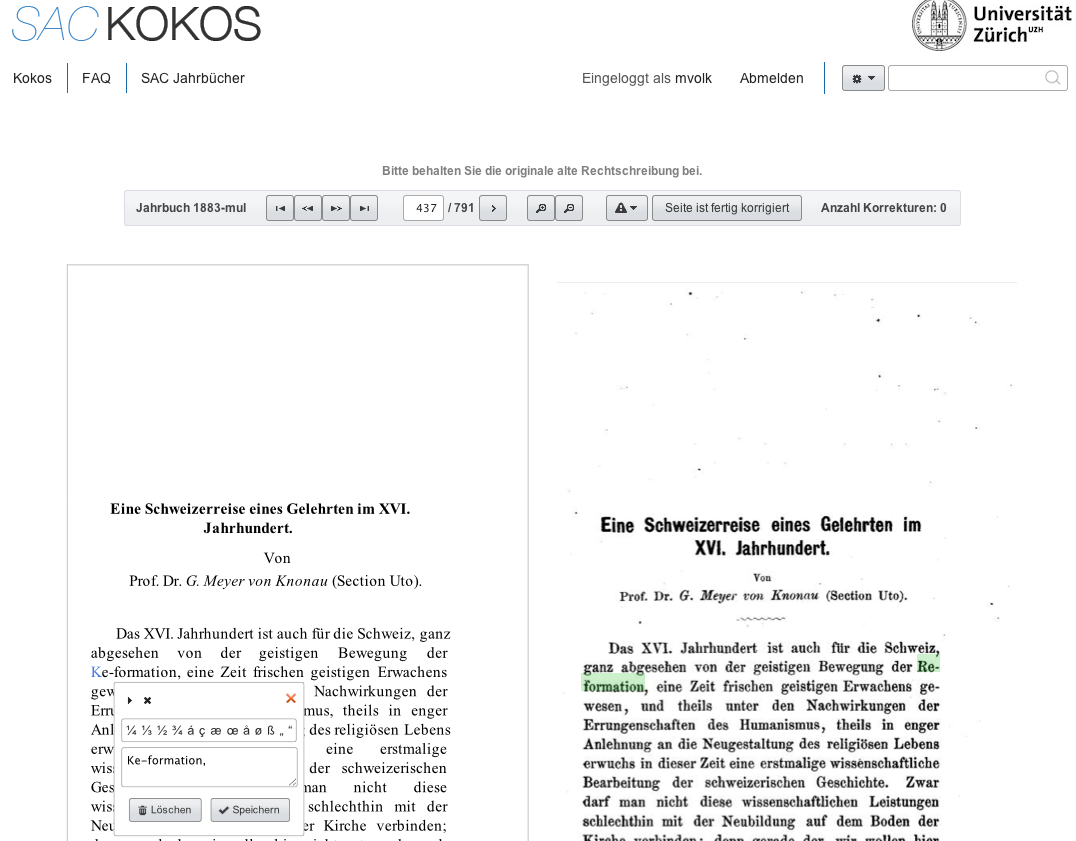
\includegraphics[height=9.5cm]{Kokos_Screen_Shot.png}
%\end{center}
%\caption{Beschreibung Kokos} \label{Kokos_screen}
%\end{figure*}

\cite{*}

\bibliographystyle{apalike}
% your bib file should go here 
\bibliography{references.G.S}


\end{document}
